%%%%%%%%%%%%%%%%%%%%%%%%%%%%%%%%%%%%%%%%%%%%%%%%%%%%%%%%%%%%%%%%%%%%%%%%%%%%%%%%
%                         FORMATO DE TESIS                              %
%%%%%%%%%%%%%%%%%%%%%%%%%%%%%%%%%%%%%%%%%%%%%%%%%%%%%%%%%%%%%%%%%%%%%%%%%%%%%%%%
% based on Harish Bhanderi's PhD/MPhil template, then Uni Cambridge
% http://www-h.eng.cam.ac.uk/help/tpl/textprocessing/ThesisStyle/
% corrected and extended in 2007 by Jakob Suckale, then MPI-iCBG PhD programme
% and made available through OpenWetWare.org - the free biology wiki
% forked from https://github.com/Tepexic/Tesis-UNAM on July 2017
% modifications made by Arturo Lopez Pineda1

%                     Under GNU License v3
% (require 'iso-transl)
% ADAPTADO PARA UMSNH:  @arturolp

\documentclass[oneside,11pt]{Latex/Classes/thesisUMSNH}
%         PUEDEN INCLUIR EN ESTE ESPACIO LOS PAQUETES EXTRA, O BIEN, EN EL ARCHIVO "PhDthesisPSnPDF.cls" EN "./Latex/Classes/"
\usepackage{blindtext}
% Para insertar texto dummy, de ejemplo, pues.
\usepackage[round, year]{natbib}  % Personalizar la bibliografía a gusto de cada quien
\bibliographystyle{unsrtnat}
 
\title{Bibliography management: \texttt{natbib} package}
\author{Share\LaTeX}
\date {}

\usepackage{titlesec}
\usepackage{enumerate}
\titlelabel{\thetitle \quad}
\usepackage{algorithm}
\usepackage{algorithmic}

%\usepackage{rotating}
\usepackage{float}
\usepackage{hyperref}


% Note:
% The \blindtext or \Blindtext commands throughout this template generate dummy text
% to fill the template out. These commands should all be removed when 
% writing thesis content.
% This file contains macros that can be called up from connected TeX files
% It helps to summarise repeated code, e.g. figure insertion (see below).

%%%%%%%%%%%%%%%%%%%%%%%%%%%%%%%%%%%%%%%%%%%%%%
%            Colores de la UNAM              %
%%%%%%%%%%%%%%%%%%%%%%%%%%%%%%%%%%%%%%%%%%%%%%
% Para UNAN: Azul Pantone 541  -->(0,63,119) RGB
% Para UMSNH: PANTONE Blue 072 C
\definecolor{Vino}{RGB}{089,035,033}

% Para UNAM: Oro Pantone 460  -->(234,221,150) RGB
% Para UMNSH: PANTONE 110 C
\definecolor{Gris}{RGB}{156,156,156}


%%%%%%%%%%%%%%%%%%%%%%%%%%%%%%%%%%%%%%%%%%%%%%
%            Comandos para líneas            %
%%%%%%%%%%%%%%%%%%%%%%%%%%%%%%%%%%%%%%%%%%%%%%
%Se define un comando \colorvrule para hacer líneas verticales de color con 3 argumentos: color, ancho, alto
\newcommand{\colorvrule}[3]{
\begingroup\color{#3}\vrule width#2 height#3
\endgroup}

%Se define un comando \colorhrule para hacer líneas horizontales de color con 2 argumentos: color, ancho
\newcommand{\colorhrule}[2]{
\begingroup\color{#3}\hrule height#2
\endgroup}

%%%%%%%%%%%%%%%%%%%%%%%%%%%%%%%%%%%%%%%%%%%%%%
%          Comando para derivadas            %
%%%%%%%%%%%%%%%%%%%%%%%%%%%%%%%%%%%%%%%%%%%%%%
\newcommand{\derivada}[3][]{\ensuremath{\dfrac{\mbox{d}^{#1}#2}{\mbox{d}#3^{#1}}}} 
%primer argumento(opcional): orden de la derivada
%segundo argumento: función a derivar
%tercer argumento: variable respecto a la que se deriva


%%%%%%%%%%%%%%%%%%%%%%%%%%%%%%%%%%%%%%%%%%%%%%
%       Comando para la exponencial          %
%%%%%%%%%%%%%%%%%%%%%%%%%%%%%%%%%%%%%%%%%%%%%%
\newcommand{\e}[1][]{\ensuremath{\mbox{e}^{#1}}}
%primer argumento(opcional): exponente de la exponencial




% insert a centered figure with caption and description
% parameters 1:filename, 2:title, 3:description and label
\newcommand{\figuremacro}[3]{
	\begin{figure}[htbp]
		\centering
		\includegraphics[width=1\textwidth]{#1}
		\caption[#2]{\textbf{#2} - #3}
		\label{condicion}
	\end{figure}
}

% insert a centered figure with caption and description AND WIDTH
% parameters 1:filename, 2:title, 3:description and label, 4: textwidth
% textwidth 1 means as text, 0.5 means half the width of the text
\newcommand{\figuremacroW}[4]{
	\begin{figure}[htbp]
		\centering
		\includegraphics[width=#4\textwidth]{#1}
		\caption[#2]{\textbf{#2} - #3}
		\label{#1}
	\end{figure}
}

% inserts a figure with wrapped around text; only suitable for NARROW figs
% o is for outside on a double paged document; others: l, r, i(inside)
% text and figure will each be half of the document width
% note: long captions often crash with adjacent content; take care
% in general: above 2 macro produce more reliable layout
\newcommand{\figuremacroN}[3]{
	\begin{wrapfigure}{o}{0.5\textwidth}
		\centering
		\includegraphics[width=0.48\textwidth]{#1}
		\caption[#2]{{\small\textbf{#2} - #3}}
		\label{#1}
	\end{wrapfigure}
}

% predefined commands by Harish
\newcommand{\PdfPsText}[2]{
  \ifpdf
     #1
  \else
     #2
  \fi
}

\newcommand{\IncludeGraphicsH}[3]{
  \PdfPsText{\includegraphics[height=#2]{#1}}{\includegraphics[bb = #3, height=#2]{#1}}
}

\newcommand{\IncludeGraphicsW}[3]{
  \PdfPsText{\includegraphics[width=#2]{#1}}{\includegraphics[bb = #3, width=#2]{#1}}
}

\newcommand{\InsertFig}[3]{
  \begin{figure}[!htbp]
    \begin{center}
      \leavevmode
      #1
      \caption{#2}
      \label{#3}
    \end{center}
  \end{figure}
}







%%% Local Variables:
%%% mode: latex
%%% TeX-master: "~/Documents/LaTeX/CUEDThesisPSnPDF/thesis"
%%% End:
           % Archivo con funciones útiles





%%%%%%%%%%%%%%%%%%%%%%%%%%%%%%%%%%%%%%%%%%%%%%%%%%%%%%%%%%%%%%%%%%%%%%%%%%%%%%%%
%                                   DATOS                                      %
%%%%%%%%%%%%%%%%%%%%%%%%%%%%%%%%%%%%%%%%%%%%%%%%%%%%%%%%%%%%%%%%%%%%%%%%%%%%%%%%
\title{An\'alisis de datos gen\'eticos en población mexicana y su relación con el c\'ancer colorrectal}
\author{Edison Jessie Vázquez Gordillo} 
\facultad{Unidad Monterrey}                 % Nombre de la facultad/escuela
\escudofacultad{Latex/Classes/Escudos/cimat-mty} % Aquí ponen la ruta y nombre del escudo de su facultad, actualmente, la carpeta Latex/Classes/Escudos cuenta con los siguientes escudos:
% "fi_azul" Facultad de ingenieria en color azul
% "fi_negro" Facultad de ingenieria en color negro
% "fc_azul" Facultad de ciencias en color azul
% "fc_negro" Facultad de ciencias en color negro
% Se agradecen sus aportaciones de escudos a jebus.velazquez@gmail.com

\degree{Maestro en Cómputo Estadístico}       % Carrera
\director{Dr. Rodrigo Macías Páez}% Director de tesis
\tutor{Dr. Augusto Rojas Mart\'inez}
%\tutor{Nombre  Tutor }                    % Tutor de tesis, si aplica
\degreedate{2018}                                     % Año de la fecha del examen
\lugar{Monterrey, Nuevo León}                        % Lugar

%\portadafalse                              % Portada en NEGRO, descomentar y comentar la línea siguiente si se quiere utilizar
\portadatrue                                % Portada en COLOR



%Opciones del posgrado (descomentar si las necesitan)
	%\posgradotrue                                                    
	%\programa{programa de maestría en cómputo estadístico}
	%\campo{Ciencia de datos}
	%% En caso de que haya comité tutor
	%\comitetrue
	%\ctutoruno{Dr. Emmet L. Brown}
        %\ctutordos{Dr. El Doctor}
%Datos del jurado                             
	%\presidente{Dr. 1}
	%\secretario{Dr. 2}
	%\vocal{Dr. 3}
	%\supuno{Dr. 4}
	%\supdos{Dr. 5}
	%\institucion{Centro de Investigación, Unidad Monterrey}

\keywords{Genómica,Ancestria,Cáncer colo rectal}            % Palablas clave para los metadatos del PDF
\subject{tema_1,tema_2}                     % Tema para metadatos del PDF  

\titleformat{\section}[block]
{\normalfont\large\bfseries}{\thesection}{1em}{}
\titlespacing*{\subsection}
{5pt}{3.25ex plus 1ex minus .5ex}{1.5ex plus .5ex}

%%%%%%%%%%%%%%%%%%%%%%%%%%%%%%%%%%%%%%%%%%%%%%%%%%%%%
%                   PORTADA                         %
%%%%%%%%%%%%%%%%%%%%%%%%%%%%%%%%%%%%%%%%%%%%%%%%%%%%%
\begin{document}


\renewcommand{\bibname}{Bibliograf\'ia}
\renewcommand{\contentsname}{Contenido}
\renewcommand{\listfigurename}{Lista de Figuras}
\renewcommand{\listtablename}{Lista de Tablas}

\maketitle									% Se redefinió este comando en el archivo de la clase para generar automáticamente la portada a partir de los datos



%%%%%%%%%%%%%%%%%%%%%%%%%%%%%%%%%%%%%%%%%%%%%%%%%%%%%
%                  PRÓLOGO                          %
%%%%%%%%%%%%%%%%%%%%%%%%%%%%%%%%%%%%%%%%%%%%%%%%%%%%%
\frontmatter
\begin{dedication}
A Dios por la oportunidad de cumplir este sueño. A mis padres, Hortencio y Maria Elena, por su apoyo incondicional y sus esfuerzos por tener una educacion. A mi prometida Jenny, por su comprensi\'on y sus palabras de aliento que me motivar\'on a cada instante. 
\end{dedication}
       % Comentar línea si no se usa
%\chapter*{}
%\pagenumbering{Roman}

\begin{acknowledgements}

  Primeramente agradezco al Centro de Investigaci\'on en Matem\'aticas Unidad Monterrey por haberme aceptado ser parte de esta gran instituci\'on y abierto sus puertas de su seno cient\'ifico para poder realizar mis estudios de posgrado, as\'i mismo a los docentes que brindaron sus conocimientos y su apoyo para seguir adelante en cada escal\'on de este desafio.\\

  Agradezco tambi\'en al CONACyT por el apoyo econ\'omico otorgado para la realizaci\'on de este programa de maestr\'ia.\\

  Mi agradecimiento tambi\'en a mis asesores de tesina, al Dr. Rodrigo Mac\'ias por su apoyo y su conocimiento entregado. Al Dr. Augusto Rojas Mart\'inez y la Dra. Roc\'io Ortiz L\'opez por la oportunidad de participar en esta investigaci\'on.\\

  Y para finalizar, tambi\'en agradezco a todos los que fueron mis compañeros de clases durante esto dos años de programa, ya que gracias a la amistad de ustedes los d\'ias mas dificiles se pudieron pasar con alegr\'ia. 

\end{acknowledgements}




   % Comentar línea si no se usa 
% ******************************* Thesis Declaration ********************************

\begin{declaration}

Por la presente declaro que, salvo cuando se haga referencia específica al trabajo de otras personas, el contenido de esta tesina es original y no se ha presentado total o parcialmente para su consideración para cualquier otro título o grado en esta o cualquier otra Universidad. Esta tesina es resultado de mi propio trabajo y no incluye nada que sea el resultado de algún trabajo realizado en colaboración, salvo que se indique específicamente en el texto. 
% Author and date will be inserted automatically from thesis.tex


\end{declaration}
           % Comentar línea si no se usa

% Thesis Abstract -----------------------------------------------------


%(require 'iso-transl)
%\begin{abstractslong}    %uncommenting this line, gives a different abstract heading
\begin{abstracts}        %this creates the heading for the abstract page

En la actualidad se han generado bases de datos gen\'omicas para el estudio de la relaci\'on de las variantes gen\'eticas humanas y enfermedades; esto implica tratar con bases de datos de alta dimensionalidad provocando problemas a la hora de realizar an\'alisis computacionales y estad\'isticos que nos permitan entender la poblaci\'on bajo estudio. En este trabajo de titulación se realiza una revisi\'on de literatura, aplicaci\'on de m\'etodos computacionales y modelos estad\'isticos que nos ayuden a obtener resultados \'optimos en todos los sentidos, tanto como en el \'area de la computación y la medicina.

Se obtuvier\'on gr\'aficas de color que nos muestran el porcentaje de ancestralidad de las poblaciones mexicana (MXL), africana (YRI) y española (IBS), donde se obtuvo que dos de las cuatro variantes de nucle\'otido simple (SNPs) tienen mayor porcentaje de ancestralidad europea (española) lo cual puede dar indicio de una relaci\'on entre esta poblaci\'on geogr\'afica y el c\'ancer colorrectal.

Con los resultados y la metodolog\'ia llevada a cabo se gener\'o en M\'exico un antecedente computacional que permita recrear estos an\'alisis g\'eneticos poblaciones en otro tipos de enfermedades y observar el comportamiento y el impacto poblacional en enfermedades cr\'onicas.  

\end{abstracts}
%\end{abstractlongs}


% ----------------------------------------------------------------------
                   % Comentar línea si no se usa


%%%%%%%%%%%%%%%%%%%%%%%%%%%%%%%%%%%%%%%%%%%%%%%%%%%%%
%                   ÍNDICES                         %
%%%%%%%%%%%%%%%%%%%%%%%%%%%%%%%%%%%%%%%%%%%%%%%%%%%%%
%Esta sección genera el índice
\setcounter{secnumdepth}{3} % organisational level that receives a numbers
\setcounter{tocdepth}{4}    % print table of contents for level 3
\tableofcontents            % Genera el índice 
%: ----------------------- list of figures/tables ------------------------


%%%%%%%%%%%%%%%%%%%%%%%%%%%%%%%%%%%%%%%%%%%%%%%%%%%%%
%                   CONTENIDO                       %
%%%%%%%%%%%%%%%%%%%%%%%%%%%%%%%%%%%%%%%%%%%%%%%%%%%%%
% the main text starts here with the introduction, 1st chapter,...
\mainmatter
\def\baselinestretch{1.5}                   % Interlineado de 1.5

% this file is called up by thesis.tex
% content in this file will be fed into the main document
%----------------------- introduction file header -----------------------
%%%%%%%%%%%%%%%%%%%%%%%%%%%%%%%%%%%%%%%%%%%%%%%%%%%%%%%%%%%%%%%%%%%%%%%%%
%  Capítulo 1: Introducción- DEFINIR OBJETIVOS DE LA TESIS              %
%%%%%%%%%%%%%%%%%%%%%%%%%%%%%%%%%%%%%%%%%%%%%%%%%%%%%%%%%%%%%%%%%%%%%%%%%
%(require 'iso-transl)



\chapter{Introducci\'on y objetivo del trabajo}

%: ----------------------- HELP: latex document organisation
% the commands below help you to subdivide and organise your thesis
%    \chapter{}       = level 1, top level
%    \section{}       = level 2
%    \subsection{}    = level 3
%    \subsubsection{} = level 4
%%%%%%%%%%%%%%%%%%%%%%%%%%%%%%%%%%%%%%%%%%%%%%%%%%%%%%%%%%%%%%%%%%%%%%%%%
%                           Presentación                                %
%%%%%%%%%%%%%%%%%%%%%%%%%%%%%%%%%%%%%%%%%%%%%%%%%%%%%%%%%%%%%%%%%%%%%%%%%


Esta tesina se centra en el tema de la ancestría genética en población mexicana y su relaci\'o con el cáncer colorrectal. Como este tema en concreto no está analizado en la literatura especializada, el principal objetivo de este trabajo es dar una visión de la problemática y presentar el análisis computacional desarrollado. \\

La problem\'atica computacional implicada en estos tipos de estudios est\'a relacionada con el gran tamaño del conjunto de datos (volumen) y a su complejidad (alta dimensi\'on), la cuales dificultan su captura, gestión, procesamiento o análisis mediante técnologías y herramientas computacionales. Por lo tanto, en forma específica, esta tesina tiene como objetivo final definir la relación de ancestría de los genes con la suceptibilidad del desarrollo de cáncer colorrectal a través de métodos computacionales y estadísticos de alto rendimiento. En este trabajo vamos a analizar la ancestría poblacional del grupo a estudiar, obteniendo el porcentaje de genes pertenecientes a una región en especifico y comparar las regiones de genes susceptibles al cáncer colorrectal con las regiones de genes del grupo estudiado, para determinar si hay un vínculo entre la ancestría de estos genes con el desarrollo del cáncer.\\


Para conseguir estos objetivos se presenta una descripción breve de lo que es el análisis de ancestría genética y sus dependencia o problem\'atica en relación al desarrollo de cáncer. Posteriormente, para definir el porcentaje de ancestría de genes de la población a estudiar, se establecer\'an los marcadores informativos de ancestría (AIMs) que indican a que región geográfica pertenece cada gen. Por último, enfocaremos el estudio de los métodos para el análisis computacional y estadístico que apoye a lograr el objetivo final. \\

Así, la finalidad de este tesina es el de lograr generar antecendentes en el estudio de ancestría genética y su relación con el desarrollo de enfermedades cancerígenas y el análisis óptimo de los datos provenientes de estos estudios.\\

% estadistica cancer y la mortandad

En la actualidad, en el mundo se estima alrededor de 38 millones de muertes anuales, de las cuáles el 63\% de estas difunciones son a causa de enfermedades no transmisibles (ENT) que generalmente son crónicas y de larga duración ya que progresan lentamente. Los cuatro tipos de mayor importancia son las enfermedades cardiovasculares, las enfermedades crónicas, la diabetes y el \textbf{cáncer} \cite{INEGI}.\\

% hablar cosbre el cancer colo rectal

El cáncer de colon y recto es el cuarto cáncer m\'as frecuente en México y a nivel mundial. De los 38 millones de muerte por las ENT, casi un millón de estas muertes son causadas por este cáncer \cite{INSP}. Además representa el 2.68\% de todos los tumores malignos \cite{Dario}. \\

% los impactos ambientales y los geneticos en el cancer

Por otro lado, las enfermedades crónico-degenarativas como el cáncer, pueden tener relación de desarrollo con los agentes ambientales \cite{Weinberg} y con variantes gen\'eticas. \\

Por tanto, en la conceptualizaci\'on del problema, existen cuatro puntos a considerar: \\

\begin{enumerate}[(1)]
\item Las variantes gen\'eticas est\'an implicadas en la susceptibilidad al c\'ancer.
\item Las variantes gen\'eticas en una poblaci\'on dependen de los flujos gen\'eticos que han ocurrido durante las migraciones y los procesos de selecci\'on natural a las que se han sometido las poblaciones actuales.
\item En el caso de M\'exico, se dio un proceso historico de mezcla de por lo menos tres poblaciones humanas ancestrales: nativo americano, española y africana.
\item El proceso de mestizaje se caracteriza por la coexistencia de variantes gen\'omicas ancestrales que puedan tener un afecto en la susceptibilidad al c\'ancer colorrectal.
\end{enumerate}

%plantear la pregunta medica de ancestralidad
En este contexto, se presenta la primera pregunta a contestar: \textit{¿Hay relación de la ancestr\'ia de genes con la suceptibilidad al c\'ancer colorrectal?}.\\

%hablar sobre la complejidad de los datos de genetica

En la misma línea del análisis génetico poblacional y su relación con el cáncer colorrectal, se plantea la problem\'atica de la complejidad de la información. Los datos del genoma humano presentan secuencias de variantes g\'eneticas tipo SNP en  alrededor de \textit{5-8 millones por genoma}, implicando gran cantidad de reserva en memoria de cualquier computador \cite{Beatriz}. Este proceso se basa en un esfuerzo de alta magnitud al la hora de procesar o evaluar la evolución, escabilidad y dimensionalidad de las redes transcripcionales de genes \cite{Paulino}.\\

Los problemas comunes en los estudios de génetica, con respecto al rendimiento de los métodos computacionales y técnicas estadísticas, citando a \cite{Domingo}, son:\\

\begin{itemize}
\item \textbf{El tiempo de procesamiento}, el cual suele ser elevado al tener que analizar grandes cantidades de datos.
\item \textbf{Las variables utilizadas}, son de difícil determinación e influyen considerablemente en el resultado final.
\item \textbf{La medida de asociación}, que es utilizada para el agrupamiento y condiciones, la cual suele ser de gran magnitud. 
\item \textbf{La evaluación} final de los datos y sus interpretación.
\end{itemize}\\

%planter la pregunta del problema en cuestion computacional

Por tanto, la segunda pregunta para esta investigación es \textit{¿Hay capacidad de herramientas computacionales para el procesamiento de los datos complejos y el análisis óptimo de los mismos?}.\\

En el marco de la investigación de la génetica de población, realizar este estudio dará una panaroma m\'as amplio en el tratamiento del cáncer colorrectal, de manera similar, sera un antecedente en estudios de ancestralidad en México para diferentes enfemerdades complejas, además de lograr resultados con aplicación real en este tipo de cáncer.\\

Por otro lado, la necesidad de comprender grandes y complejos conjuntos de datos, principalmente en el área de la gen\'etica, desarrollará una habilidad de extraer conocimiento útil y actuar en consecuencia a este conocimiento extraído, para mejorar los procesos computacionales y estadísticos al momento de evaluar y procesar la información.\\

El cómputo estadístico es un campo que permitirá, aunado con especialistas en el área a donde se enfoque, a la construcción de nuevos procesos de analisís de datos de alta complejidad en función a los objetivos propuestos.\\

Así pues, este trabajo de investigaci\'on tiene como objetivo principal determinar la asociación entre el c\'ancer colorrectal y la ancestr\'ia de genes por medio de herramientas estad\'isticas computacionales y evaluaciones m\'edicas.\\

Por tanto, los objetivos especifícos se dividen en dos \'areas:\\

\begin{itemize}
\item \textbf{Génomica}:
  \begin{itemize}
  \item Encontrar el procentaje de ancestr\'ia de las regiones geogr\'aficas en los individuos del grupo con la enfermedad.
  \item Revisar las regiones cromos\'omicas asociadas con el desarrollo del cáncer colo rectal e identificarlas en los genes de los individuos caso control.
  \item Identificar la ancestr\'ia de los genes que tuvieron mayor implicación con las regiones cromos\'omicas asociadas a la enfermedad.
  \end{itemize}
\item \textbf{Cómputo estadístico:}
  \begin{itemize}
  \item Comparar softwares computacionales para la lectura y procesamiento de la base de datos génomicos
  \item Desarrollar mapas de color para la visualización de la ancestr\'ia de lo genes de cada individuo
  \end{itemize}
\end{itemize}%% Organizacion

El contenido de esta investigación se encuentra dividido en los siguientes cap\'itulos:\\

\textbf{Trabajos previos.} Se introducen algunos trabajos que se han generado en el \'area de gen\'omica problacional con respecto a la relaci\'on de ancestria individual y enfermedades cr\'onicas. Adem\'as se describen los procedimientos metodol\'ogicos y los resultados que estos han encontrado en sus investigaciones. \\

\textbf{Conceptos t\'ecnicos y software ADMIXTURE y tratamiento computacional de los datos.} Se describen las bases teóricas del software computacional a utilizar. De manera similar, se definen algunos conceptos en el \'area de gen\'omica poblacional con respecto a la estimaci\'on de la ancestr\'ia y el tratamiento de los datos.\\ 

\textbf{Elementos probab\'ilisticos y metodolog\'ia.} Se describe los m\'etodos computacionales y estad\'isticos que tienen como base el software ADMIXTURE que se usan para la estimaci\'on para el valor \textbf{K} y la ancestr\'ia individual de la poblaci\'on estudiada. \\

\textbf{Resultados.} Se presenta los resultados del análisis, cuáles han sido el porcentaje de ancestría de genes en la población estudiada y además presentar la relación existente o no con el desarrollo del cáncer colorrectal.\\

\textbf{Conclusiones y futuros trabajos.} Se visualizará el proceso de la discusión de los resultados y se realizan las conclusiones y recomendaciones del proyecto de investigación e investigaci\'on futura.\\





            % ~10 painas - Explicar el propósito de la tesis
\include{Capitulo2.1/Preeliminares}


%%%%%%%%%%%%%%%%%%%%%%%%%%%%%%%%%%%%%%%%%%%%%%%%%%%%%%%%%%%%%%%%%%%%%%%%%
%           Capítulo 2: MARCO TEÓRICO - REVISIÓN DE LITERATURA
%%%%%%%%%%%%%%%%%%%%%%%%%%%%%%%%%%%%%%%%%%%%%%%%%%%%%%%%%%%%%%%%%%%%%%%%%
%(require 'iso-transl)

\chapter{Conceptos t\'ecnicos, software ADMIXTURE y tratamiento computacional de los datos}


%%%%%%%%%%%%%%%%%%%%%%%%%%%%%%%%%%%%%%%%%%%%%%%%%%%%%%%%%%%%%%%%%%%%%%%%%%%%%%%%%%%%%%%%%%%%%%%%%%%%%%%%%%%%%%%%%%%%%%%%%%%%%%%%%%%%%%%%%%%%%%%%%%%%%%%%%%%%%%%%%%%%%%%%%%%%%%%%%%%%%%%%%%%%%%%%%%%%%%%%%%%%%%%%%%%%%%%%%%%%%%%%%%%%%%%%%%%%%%%%

A continuación se presentan las bases teóricas que sustentan la investigación sobre el uso de los métodos computacionales y los métodos estadísticos para el análisis de los datos, y la identificación de la relación de ancestría con el cáncer colorrectal. También una descripci\'on breve del c\'ancer colorrectal y la estructura gen\'etica de M\'exico.\\

\section{Proceso del c\'ancer colorrectal}

El c\'ancer en general, se origina por cambios gen\'eticos en las c\'elulas, estas a su vez son la parte b\'asica que forman los tejidos, los cuales forman los \'organos del cuerpo. En este proceso, las c\'elulas crecen y se dividen para crear nuevas c\'elulas que se dividen sin control e invaden tejidos, alterando los tejidos formando una masa, que es lo que se conoce como tumor \cite{NCI}.\\

Con respecto al origen del c\'ancer colorrectal, o tambi\'en llamado c\'ancer de colon o de recto dependiendo donde se desarrolle, la American Cancer Society \cite{ACS} menciona que la mayor\'ia de estos tipos de c\'ancer comienzan como un crecimiento llamado \textit{p\'olipo} en el revistimiento del colon o del recto como se observa en la figura \ref{fig:cancer}. Seg\'un \cite{ASCRS}, los p\'olipos son ``crecimientos anormales de tejido que sugen del capa interior o mucosa del intestino grueso (colon) y sobresalen al canal intestinal''. 

\begin{figure}[H]
  \centering
  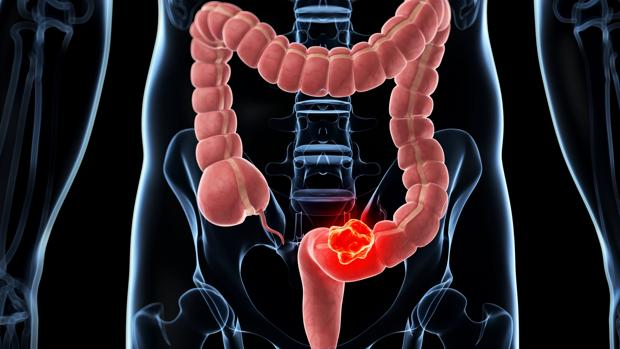
\includegraphics[scale=0.5]{cancer_colon.jpg}
  \caption[Localizaci\'on del c\'ancer colorrectal]{Localizaci\'on del c\'ancer colorrectal \cite{cancer}}
  \label{fig:cancer}
\end{figure}


En la mayoria de los casos de c\'ancer, los factores que est\'an asociados al desarrollo en estas enfermedades tienen una interacci\'on entre s\'i. En el c\'ancer colorrectal, los factores gen\'eticos y ambientales que provocan su desarrollo se favorecen por la interacci\'on de algunos de ellos como el estilo de vida, la dieta y la herencia g\'enetica. En estilos de vida, la falta de ejercicio f\'isico, el sobrepeso y la obesidad, as\'i como el consumo de tabaco y alcohol, son comunes en casos con este tipo de c\'ancer. De manera similar, existe relaci\'on con el consumo de carnes rojas, carne procesada y carne expuesta al fuego directamente, aunque no se ha determinado de que manera los alimentos ricos en fibra, vegetales y leche fungen como protectores ante este tipo de c\'ancer \cite{cancer}. La herencia, representa entre un 20 a un 25\% de los factores de riesgo para esta enfermedad \cite{Riestra}. De manera similar, el c\'ancer colorrectal tiene una prevalencia en individuos mayores a 50 años, siendo esto uno de los mayores riesgos de padecer esta enfermedad. \\



\section{Estructura gen\'etica de la poblaci\'on mexicana}

M\'exico es un pa\'is ubicado en Am\'erica del Norte  y es el tercer pa\'is m\'as grande de Am\'erica Latina. Al d\'ia de hoy, el pa\'is esta conformado por 110 grupo \'etnicos que componen la mayor parte de la poblaci\'on como se muestra en la figura \ref{fig:indigena}. La poblaci\'on de meztizos en M\'exico es de gran proporci\'on seg\'un los datos del \cite{INEGI}. En general, el concepto de \textit{mestizo} en M\'exico es para referirse  personas con una aparencia fenot\'ipica intermedia entre los esterotipos europeos o africanos y tipos de ind\'igenas endemicos del pa\'is \cite{estrada}. \\


\begin{figure}[H]
  \centering
  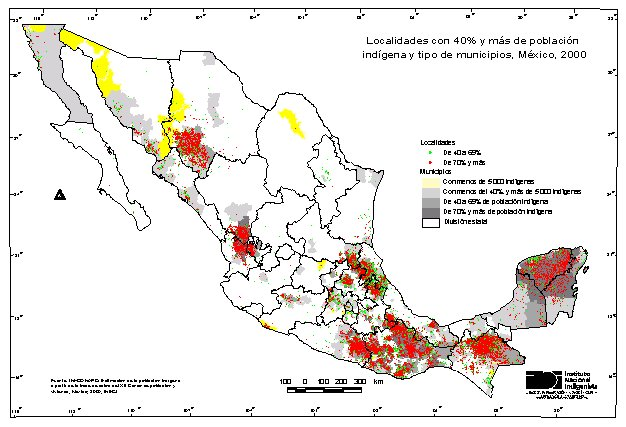
\includegraphics[scale=0.5]{mapa_003.jpg}
  \caption[Mapa de Calor para localidades ind\'igena en M\'exico]{Mapa de calor para localidades con 40\% y m\'as de poblaci\'on ind\'igena en M\'exico. El color rojo muestra las regiones con presencia ind\'igena mayor a 70\% mientras el verde representa la presencia ind\'igena menor al 40\% \cite{CNDPI}}
  \label{fig:indigena}
\end{figure}

La historia de la conquista de M\'exico empez\'o en el año 1559 cuando los europeos, sobre todo españoles, arribaron a las costas de Yucat\'an, empezando el mestizaje en esa zona, añadi\'endose individuos del \'Africa tra\'idos en esclavitud a Am\'erica. Por lo tanto, la mezcla gen\'etica entre los americanos nativos (ind\'igenas), europeos (españoles) y africanos que se produjo en M\'exico form\'o una poblaci\'on mestiza con variadas caracter\'isticas f\'isicas \cite{carlos, Gabriela} como se observa en las siguientes figuras \ref{fig:indi} y \ref{fig:calor}. \\


\begin{figure}[H]
  \centering
  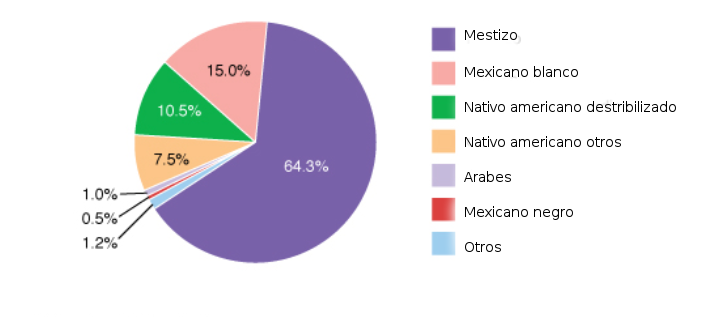
\includegraphics[scale=0.5]{etnia.png}
  \caption[Porcentaje de poblaciones por origen gen\'etico en M\'exico]{Porcentaje de poblaciones por origen gen\'etico en M\'exico \cite{Cat} }
  \label{fig:indi}
\end{figure}


\begin{figure}[H]
  \centering
  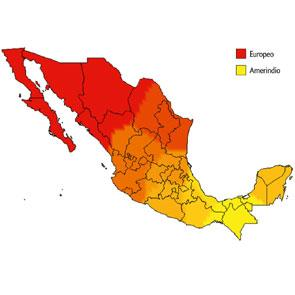
\includegraphics[scale=0.7]{calor_indi.jpg}
  \caption[Mapa de calor de dos poblaciones (europeo y americano nativo)]{Mapa de calor de dos poblaciones con origen gen\'etico europeo y americano nativo \cite{Gabriela}}
  \label{fig:calor}
\end{figure}

\section{Genotipado}\label{sub:geno}

La Academia Europea de Pacientes \cite{ACP} define el genotipado como ``el proceso mediante el cual se determinan las diferencias en los caracteres genéticos o el genotipo de un individuo mediante el análisis de su secuencia de ADN individual. Esto se puede hacer mediante la comparación del genotipo con la secuencia de otro individuo o con una secuencia de referencia''. En otras palabras, el genotipado es la t\'ecnica de laboratorio que se utiliza para determinar la informaci\'on g\'enetica de un organismo, o genotipo, y poder individualizar del resto, as\'i como la susceptibilidad y variantes causales a una enfermedad.\\


Las bases de datos que capturan el genotipado se encuentran en formato \textit{.ped} y \textit{.map} y de un archivo en formato \textit{.xlsx} que muestra los SNPs asociados a la enfermedad. Los archivos .ped describen los individuos y los datos gen\'eticos de la poblaci\'on estudiada. Este archivo puede ser delimitado por \textit{ESPACIOS} o \textit{TAB}, cada l\'inea corresponde a un solo individuo como se puede observar en la siguiente tabla.\\

 \begin{table}[H]
\centering
\begin{tabular}{|1|1|1|1|1|1|1|1|1|1|1|1|1|}
\hline \hline
FAM 1 & IND1 & 0 & 0 & 1 & 0 &  A & A & T & T & 0 & 0 & ...\\
\hline
FAM 2 & IND2 & 0 & 0 & 1 & 0 &  A & G & T & C & T & A & ... \\
\hline
FAM 3 & TRIOF & 0 & 0 & 1 & 0 & A & G & T & C & A & T & ... \\
\hline
FAM 4 & TRIOM & 0 & 0 & 2 & 0 &  A & G & T & C & A & T & ... \\
\hline
FAM 5 & TRIOC & TRIOF & TRIOF & 1 & 0 &  A & A & C & T & A & T & ... \\
\hline \hline
\end{tabular}
\caption{Ejemplo estructura datos .ped}
\label{tabla:ped}
\end{table}

 Las primera seis columnas son: \\

 \begin{enumerate}[1.]
 \item Family ID [\texit{string}]
 \item Individual ID [\texit{string}]
 \item Father ID [\texit{string}]
 \item Mother ID [\texit{string}]
 \item Sex [\texit{integer}]
 \item Phenotype [\texit{float}]
 \end{enumerate}

 Las columnas 7 y 8 codifican los alelos observados en SNP1, las columnas 9 y 10 codifican los alelos observados en SNP2, y así sucesivamente. Los datos faltantes se codifican como "0 0". Este archivo debe tener N líneas y 2L + 6 número de columnas, donde N y L son los números de individuos y SNP contenidos en el conjunto de datos, respectivamente. Es importante resaltar que cada individuo debe tener una identificación única que contenga solo caracteres alfanuméricos.\\

 Por otro lado, el archivo .map describe los SNPs. La estructura de esta informaci\'on se puede observar en la tabla \ref{tabla:map}.\\

 \begin{table}[H]
\centering
\begin{tabular}{|1|1|1|1|}
\hline \hline
7 & SNP1 & 0 & 123\\
\hline
7 & SNP3 & 0 & 456 \\
\hline
7 & SNP3 & 0 & 789\\
\hline \hline
\end{tabular}
\caption{Ejemplo de estructura de datos .map}
\label{tabla:map}
 \end{table}

 De manera similar, este archivo puede estar delimitado por ESPACIOS o TAB. Cada l\'inea corresponde a los SNPs y las cuatro columnas son:\\

 
 \begin{enumerate}[1.]
 \item Chromosome number [\texit{integer}]
 \item SNP ID [\texit{string}]
 \item SNP genetic position (cM) [\texit{float}]
 \item SNP physical position (bp) [\texit{integer}]
 \end{enumerate}


 
 \section{An\'alisis de mezcla de poblaciones}

 El an\'alisis de mezcla de poblaciones se define, seg\'un la International Society of Genetic Genealogy \cite{ISGG}, como un m\'etodo para inferir los or\'igenes geogr\'aficos de alguien basado en un an\'alisis de su ascedencia gen\'etica. La mezcla (Admixture) sucede cuando las poblaciones comienzan con el mestizaje y la desendencia de estas producen una mezcla de alelos de diferentes poblaciones ancestrales. El an\'alisis de este acontecimiento de ancestralidad tiene una importancia valiosa tanto en g\'enetica de poblaciones como en epidemiolog\'ia gen\'etica \cite{Line}.\\

 Esta t\'ecnica tiene como base la clasificaci\'on posible de los individuos en series de grupos \'etnicos com\'unmente identificados tales como europeos, americanos nativos, entre otros. Esto es posible mediante el uso de un SNP informativo de origen ancestral para obtener el porcentaje del genoma de un individuo que tiene un origen ancestral dado \cite{Orlando}, esto se puede observar en la figura \ref{fig:adm}.\\

 
\begin{figure}[H]
  \centering
  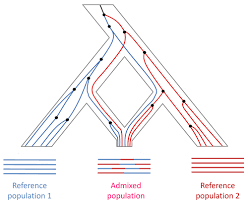
\includegraphics[scale=0.9]{images.png}
  \caption[\'Arbol de poblaci\'on y \'arbol de genes]{ Se observa el \'Arbol de población (en gris) y el árbol de genes (en azul y rojo) que rastrea la historia evolutiva de dos poblaciones ancestrales y su correspondiente población mezclada. Los haplotipos específicos de la población de referencia 1 (líneas rojas) podrían fluir y mezclarse con la población 2 y viceversa  \cite{Yuan}.}
  \label{fig:adm}
\end{figure}
 


\section{Software ADMIXTURE para la estimaci\'on de la ancestralidad}

Varios autores han usado diferentes m\'etodos para la estimaci\'on de ancestr\'ia \cite{Vero,Justo,Nuri}. Los softwares de mayor uso, especificamente diseñados para realizar \textit{admixture mapping} en la literatura son los programas \texttt{STRUCTURE}, \texttt{MALDsoft}, \texttt{ADMIXMAP}, \texttt{ANCESTRYMAP} y \texttt{ADMIXTURE}. Este \'ultimo calcula las estimaciones mucho m\'as r\'apido usando un algoritmo n\'umerico de optimizaci\'on. Especificamente ADMIXTURE es un software para la estimación de máxima verosimilitud de ancestros individuales de conjuntos de datos genotipo SNP multilocus. ADMIXTURE utiliza un enfoque de relajación de bloques (\textbf{block relaxation}, ver el apartado \ref{sec:BR}) para actualizar alternativamente la frecuencia de alelos y los parámetros de la fracción ascendente. Cada actualización de bloques se maneja resolviendo una gran cantidad de problemas de optimización convexos independientes, que se abordan usando un algoritmo de programación cuadrático secuencial rápido. La convergencia del algoritmo se acelera utilizando un novedoso método de aceleración \textit{cuasi Newton} \ref{sec:cn}. El algoritmo supera a los algoritmos EM y los métodos de muestreo MCMC por un amplio margen \cite{Admixture}. Una descripción general de los programas para la estimaci\'on de ancestr\'ia se presenta en la tabla \ref{tabla:sofadm}. \\


\begin{table}[htbp]
  \centering
\begin{tabular}[t]{|1|p{0.3\linewidth}|p{0.4\linewidth}|}
  \hline 
  \multicolumn{1}{|c|}{\textbf{Programa}} & \multicolumn{1}{c|}{\textbf{Global/local}} & \multicolumn{1}{c|}{\textbf{M\'etodo principal}} \tabularnewline \hline
  STRUCTURE & Global/Local & MCMC:Markov Chain Monte Carlo\tabularnewline \hline
frappe &Global&	ML: Maximum likelihood\tabularnewline \hline
ADMIXTURE&Global& EM: Expectation Maximization \tabularnewline \hline
EIGENSTRAT/smartpca&Global&PCA: Principal Component Analysis\tabularnewline \hline
ipPCA/EigenDev&Global&PCA: Principal Component Analysis\tabularnewline \hline
GEMTools&Global& Spectral graph\tabularnewline \hline
PLINK&Global&EM: Expectation Maximization \tabularnewline \hline
LAMP&Local/Global&Hierarchical Hidden Markov Model\tabularnewline \hline
HAPMIX&Local/Global&Infinite hidden Markov model  \tabularnewline \hline
ANCESTRYMAP&Local/Global&Bayesian and ML \tabularnewline \hline

\end{tabular}
\caption[Softwares para la estimaci\'on de ancestr\'ia]{Descripci\'on de softwares  para la estimaci\'on de ancestria local o globlal \cite{Yushi}}
\label{tabla:sofadm}
\end{table}

A grandes rasgos, el software ADMIXTURE estima la probabilidad para los genotipos observados basandose en las proporciones de ascedencia y frecuencias de alelos de poblaci\'on, realiz\'andolo simultaneamente. El archivo de entrada debe de representar a los genotipos de individuos no relacionados, el cual puede ser una estimaci\'on del número de poblaciones \texttt{K}.\\ 

Ahora bien, para la estimaci\'on de la ancestr\'ia ADMIXTURE enfoca sus estimaciones en el m\'etodo de m\'axima verosimilitud (EM) (ver \ref{sec:EM}), en lugar de los m\'etodos tradicionales para estos tipos de estudio como muestrear la distribuci\'on posterior utilizando MCMC. Adem\'as, con el m\'etodo de block relaxation aumenta la velocidad de la estimaci\'on haciendo que sea superior en eficiencia computacional respecto a otros programas de alto nivel como STRUCTURE. En l\'ineas generales, ADMIXTURE actualiza el par\'ametro de frecuencia del alelo y el par\'ametro de fracci\'on ascendente alternativamente maximizando la expansi\'on de la funci\'on de verosimilitud de Taylor de segundo orden. Para realizar este proceso se usa programaci\'on cuadr\'atrica secuencial y se desarrolla de manera iterativa en funci\'on de las frecuencias de los alelos y las proporciones de ascendencia asociadas con los valores de los par\'ametros actuales.Dado que es iterativo y se necesita encontrar un punto \'optimo para resolver $x-M(x) = 0$, el m\'etodo de Newton se puede usar para esta b\'usqueda. Sin embargo, obtener el diferencial de M(x) es desafiante, por lo que se usa un m\'etodo cuasi-Newton, lo que permite la acelaraci\'on de convergencia y tiene una ventaja sobre los m\'etodos de velocidad sobre convergencia como el m\'etodo EM. Se ha probado con datos reales y se ha encontrado que ADMIXTURE es mucho m\'as r\'apido que STRUCTURE pero con una estimaci\'on comparable \cite{Yushi}. \\

Por otro lado, existen dos denominaciones de ADMIXTURE para estimar la ancestr\'ia. La estimaci\'on de ascedencia se demonina \textbf{Supervisada} cuando se considera los genotipos de individuos con ancestros conocidos, para ello se necesita archivos \texttt{.pop}. Cuando no se incluyen individuos con ancestros conocidos entonces se denomina \txtbf{no supervisada} \cite{Timothy}.\\


\section{Estimaci\'on de ancestr\'ia por proyecci\'on}

Cuando se tiene un conjunto de datos nuevo de genes, donde se tiene como
objetivo estimar la ancestria, existe la manera de utilizar conjuntos
de datos como paneles de referencia, tales como los proyectos
\textbf{1000Genomes} o \textbf{HapMap}. Estos se usan en combinaci\'on con la
muestra del estudio para estimación de la ancestr\'ia utilizando softwares como ADMIXTURE, debido a que estos grandes conjuntos de
datos resumen la estructura de la poblaci\'on humana. Es decir, para
las muestras del estudio que no incluyen una poblaci\'on nueva, una
forma eficiente de estimar la ascedencia individual es
\textbf{proyectar} las nuevas muestras en la estructura de la poblaci\'on conocida (aprendida) de los paneles de referencia.\\

La manera en que se realiza esta operaci\'on tiene una estructura similar a la operaci\'on de proyecci\'on utilizada en el an\'alisis de componentes principales, aunque los detalles matem\'aticos difieren. Para el tipo de poyecci\'on no supervisada se requiere que las dos bases de datos (los paneles de referencia y los datos del estudio) tengan los mismos SNP's, siendo que se aprende del conjunto de datos de referencia y las proporciones de ascendencia se pueden inferir para el conjunto de datos del estudio.\\

En el aspecto matem\'atico, esto requiere resolver el problema de maximizaci\'on de verosimilitud de la ecuaci\'on 4.2, del capitulo 4, con respecto a \texttt{Q} para un \texttt{P} fijo. Este tipo de problemas son convexos y se resuelven de manera eficiente con la ayuda de los algoritmos de optimizaci\'on como Block Relaxation \cite{Suyash}.



%%%%%%%%%%%%%%%%%%%%%%%%%%%%%%%%%%%%%%%%%%%%%%%%%%%%%%%%%%%%%%%%%%%%%%%%%%%%%%%%%%%%%%%%%%%%%%%%%%%%%%%%%%%%%%%%%%%%%%%%%%%%%%%%%%%%%%%%%%%%%% %%%%%%%%%%%%%%%%%%%%%%%%%%%%%%%%%%%%%%%%%%%%%%%%%%%%%%%%%%%%%%%%%%%%%%%%%%%%%%%%%%%%%%%%%%%%%%%%


           % ~20 páginas - Poner un contexto a la tesis, hacer referencia a trabajos actuales en el tema

%%%%%%%%%%%%%%%%%%%%%%%%%%%%%%%%%%%%%%%%%%%%%%%%%%%%%%%%%%%%%%%%%%%%%%%%%
%           Capítulo 3: NOMBRE                   %
%%%%%%%%%%%%%%%%%%%%%%%%%%%%%%%%%%%%%%%%%%%%%%%%%%%%%%%%%%%%%%%%%%%%%%%%%
%(require 'iso-transl)

\chapter{Elementos probabil\'isticos y metodolog\'ia}
En este capítulo, se describe la introducción al desarollo de la tesis, los m\'etodos de computaci\'on para el procesamiento de los datos y su an\'alisis. De manera similar, los elementos probabil\'isticos para el an\'alisis de datos. 

%%%%%%%%%%%%%%%%%%%%%%%%%%%%%%%%%%%%%%%%%%%%%%%%%%%%%%%%%%%%%%%%%%%%%%%%%
%                          Descripción de la planta                     %
%%%%%%%%%%%%%%%%%%%%%%%%%%%%%%%%%%%%%%%%%%%%%%%%%%%%%%%%%%%%%%%%%%%%%%%%%


\section{Modelo probabil\'istico}

Las bases de datos t\'ipicas para la estimaci\'on de la ancestr\'ia consiste en genotipos en un gran n\'umero \texttt{J} de SNPs de un gran n\'umero \texttt{I} de individuos no relacionados. Como en cualquier parte del mundo, estos individuos provienen de una poblaci\'on mixta con contribuciones de poblaciones ancestrales postuladas por \texttt{K}. La poblaci\'on \texttt{k} contribuye con una fracci\'on $q_{ik}$ de un gemona $i's$ individual. Por lo tanto, el alelo 1 en el SNP \texttt{j} tiene la frecuencia $f_{kj}$ en la poblaci\'on \texttt{k}.\\

Puede ser que el alelo 1 sea el alelo menor y el alelo 2 sea el alelo principal o viceversa, no importa ya que esto deriva al mismo resultado. Lo que realmente importa es que tanto el la fracci\'on de contribuci\'on $q_{ik}$ y la frecuencia $f_{kj}$ son desconocidas. Por lo tanto, es necesario estimar a $q_{ik}$ para saber la ascendencia en un estudio de asociaci\'on , pero tambi\'en enfoc\'andonos en la estimaci\'on de $f_{kj}$. Esto nos permite estimar el grado de divergencia entra las poblaciones ancestrales estimadas utilizando la estad\'istica $F_{ST}$. \\

El modelo estad\'istico de likelihood que adopta ADMIXTURE viene de STRUCTURE, donde los individuos est\'an formados por la uni\'on aleatoria de gametos, lo que produce las proporciones binomiales\\

\begin{equation}
  \begin{array}{l}
  Pr(\textup{1/1 para cada i en el SNP j}) = [\sum_{k} q_{ik}f_{kj}]^{2}\\
  Pr(\textup{1/2 para cada i en el SNP j}) = 2[\sum_{k}q_{ik}f_{kj}][\sum_{k}q_{ik}(1-f_{kj})]\\
  Pr(\textup{2/2 para cada i en el SNP j}) = [\sum_{k}q_{ik}(1-f_{kj})]^{2}.
  \end{array}
  \end{equation}\\

Este modelo realiza una suposici\'on adicional de equilibrio de ligamento (linkage equilibrium) entre los marcadores. Adem\'as de que los conjuntos grandes o densos de marcadores deben ser podados con el proposito de mitigar el desequilibrio de ligamento (LD) de fondo.\\

Por otro lado, el registro de los datos se realiza por recuentos. Por lo tanto, $g_{ij}$ representa el n\'umero observado de copias de alelo 1 en el marcador \texttt{j} de la persona \texttt{i}. En consecuencia, $g_{ij}$ puede ser igual a 0,1 o 2 de acuerdo al genotipo 2/2,1/2 o 1/1 de la persona \texttt{i} en el marcador \texttt{j}. Si consideramos que los individuos son independientes, que para todos los casos as\'i se consideran, la funci\'on loglikehood de la muestra entera es\\

\begin{equation}
  L(Q,F) = \sum_{i}\sum_{j}{g_{ij}ln[\sum_{k}q_{ik}f_{kj}] + (2-g_{ij})ln[\sum_{k}q_{ik}(1-f_{kj})]}.
\end{equation}

Se observa que los par\'ametros $Q={q_{ik}}$ y $F={f_{kj}}$ con dimensiones $IXK$ y $KXJ$ respectivamente, dando un total de $K(I + J)$ par\'ametros. En un ejemplo real, si consideramos que $I=1000$, $J=10,000$ y $K=3$, se tendr\'ian que estimar alrededor de 33,000 par\'ametros. Este n\'umero hace que el m\'etodo de Newton no sea factible. El espacio requerido para la matriz hesiana es demasiado grande, y su matriz inversa de esta es computacionalmente costosa.

\section{Algoritmo de relajaci\'on de bloques} \label{sec:BR}

El algoritmo de relajaci\'on de bloques es diferente a los m\'etodos de descenso de coordenadas, los cuales tienen la gran ventaja de que conducen a problemas de optimizaci\'on unidimensional, siendo muchos m\'as sencillos que los multidimensionales. En la mayor\'ia de los casos reales tenemos problemas multidimensionales como en el \'area de la g\'enetica. A continuaci\'on se dar\'a una definici\'on breve del algoritmo de relajaci\'on de bloques(BR) \cite{deLeeuw}.\\

El m\'etodo de relajaci\'on de bloques se define matematicamente como m\'etodos de punto fijo. De manera general se da una descripci\'on de los m\'etodos de punto fijo. Se llama un punto fijo a un punto que satisface la siguiente ecuaci\'on.\\

\begin{equation}
  x=g(x)
\end{equation}

El teorema del punto fijo define a \texttt{D} como un conjunto, y busca condiciones en \texttt{D} y \texttt{g} que garantizen la existencia de \texttt{x}; condiciones que garantizan unicidad (no obligatoriamente). Para ello se puede utilizar el m\'etodo de iteracci\'on de punto fijo que se muestra en la tabla \ref{table:br}. \\


\begin{table} [H]
     \centering
  \begin{tabular}{|l|}
 
    \hline \hline
    \textbf{Algoritmo} Fixed Point Iteration \\
    \hline \hline
    
   
    \textbf{1.} Dada una ecuaci\'on f(x) = 0 \\
    
    \textbf{2.} Convertimos la ecuaci\'on f(x)=0 a la forma x = g(x)\\
    
    \textbf{3.} Damos un valor inicial aleatorio para $x_{0}$\\
    
    
    \textbf{4.} Do  \\

     \ \ \ \ \ \ \ \ \ \ \ \ \ \ \ \ \ \ \ \textbf{$x_{i+1} = g(x_{i})$}\\
 
    \textbf{5.} while(no se cumpla ninguno de los dos criterios de convergencia \texttt{C1} o \texttt{C2})\\
      
    \hline
    
  \end{tabular}
  \caption{Descripci\'on algoritmo Fixed Point Iteration}
  \label{table:br}
\end{table}


\begin{itemize}
\item \texttt{C1}: Se corrigi\'o apriori el n\'umero total de iteracciones N
\item \texttt{C2}: Al probar la condici\'on $|x_{i+1}-g(x_{i})|$ (donde \textbf{i} es el n\'umero de iteracciones) con un limite de tolerancia $\epsilon$, donde se fija el apriori. 
\end{itemize}


Entendiendo el concepto del m\'etodo punto fijo, se consider\'o la siguiente condici\'on general para el algoritmo de relajaci\'on de bloques. Se minimizo la funci\'on \textbf{f} de valor real en el conjunto de productos $X = X_{1} \otimes X_{2} \otimes ... \otimes X_{p}$, donde $X_{s} \subseteq \mathsf{R}^{n_{s}
}$  .\\

Para minimizar esta funci\'on se utiliza el siguiente m\'etodo iterativo (Tabla \ref{table:MI}, que tiene su base en el algoritmo iterativo anterior \ref{table:br}.\\

\begin{table} [H]
  \centering
  \begin{tabular} {|l|}
    \hline
    Comenzar: \ \ \ \ \ \ \ \ \ \ \ \ \ \  Empezar con $x^{(0)} \in X$ \\
    \hline
    Paso k.1:  \ \ \ \ \ \ \ \ \ \ \ \ \ \ $x_{1}^{k+1} \in \underset{x_{1} \in X_{1}}{\operatorname{argmin}} f(x_{1},x_{2}^{k},...,x_{p}^{k}).$ \\
    
    Paso k.2:  \ \ \ \ \ \ \ \ \ \ \ \ \ \  $x_{2}^{k+1} \in \underset{x_{2} \in X_{2}}{\operatorname{argmin}} f(x_{1}^{k+1},x_{2},x_{3}^{k}...,x_{p}^{k}).$ \\
    
    \ \ \ \ \ ...  \ \ \ \ \ \ \ \ \ \ \ \ \ \ \ \ \ \ \ \ \ \ \ \ \ \ \ \ \ \ \ \ ... \\
    
    Paso k.p:  \ \ \ \ \ \ \ \ \ \ \ \ \ \   $x_{p}^{k+1} \in \underset{x_{p} \in X_{p}}{\operatorname{argmin}} f(x_{1}^{k+1},...,x_{p-1}^{k+1},x_{p}).$ \\
    \hline
    Motor: k $\leftarrow$ k + 1 e ir hacia k.1 \\
    \hline
    
  \end{tabular}
  \caption{M\'etodo iterativo}
  \label{table:MI}
\end{table}

En este m\'etodo iterativo se puede observar que existen m\'inimos en la subetapas, pero no necesitan ser \'unicos (aunque se espera que esta condici\'on exista). El argumento de m\'inimo son mapas punto a punto, aunque en muchos casos se asignan en singletons (conjunto con exactamente un elemento). En los problemas reales se har\'an c\'alculos con selecci\'on del argmin.\\


\section{Acelaraci\'on de convergencia}\label{sec:cn}

Como es bien conocido, los algoritmos EM no son en su defecto de altas tasas de convergencia. De manera similar, en el esquema de relajaci\'on de bloques, aunque es m\'as r\'apido que los algoritmos EM, a\'un tiene poca potencia de convergencia, por tanto es necesario utilizar un acelador de convergencia. A continuaci\'on se describe un m\'etodo g\'enerico que se us\'o junto con el software ADMIXTURE \cite{}.\\

Se supone que un algoritmo est\'a definido por un mapa de iteraci\'on $x^{n+1} = M(x^{n})$. Dado que el punto \'optimo es un punto fijo del mapa de iteraci\'on, uno puede intentar encontrar el punto \'optimo aplicando el m\'etodo de Newton a la ecuaci\'on $x-M(x)=0$. Debido a que la diferencial $dM(x)$ muestra resistencia al computar, entonces los m\'etodos cuasi-Newton buscan aproximarlo mediante condiciones secantes que involucran repeticiones previas. Para mantener la complejidad computacional bajo control, se limita el n\'umero de condiciones de la secante durante la aceleraci\'on, as\'i evitando un sobreajuste de operaciones. Adem\'as este m\'etodo tiene las ventajas de evitar el almacenamiento y la inversión de matrices grandes y preservar las restricciones lineales de igualdad. Para mantener la complejidad computacional bajo control, se limit\'o el número de condiciones de la secante durante la aceleración. La propiedad de ascenso del algoritmo EM y la relajación del bloque son útiles para monitorear la aceleración. Cualquier paso acelerado que lleve cuesta abajo es rechazado a favor de un paso ordinario. Los pasos acelerados no dependen necesariamente de las restricciones, por lo que las actualizaciones de los parámetros están cayendo fuera de sus regiones factibles \cite{Zhou2011}.

\section{Algoritmo EM} \label{sec:EM}

A trav\'es del programa de ADMIXTURE se us\'o el algoritmo EM de FRAPPE que b\'asicamente actualiza los par\'ametros a trav\'es de lo siguiente: \\

\begin{equation}
  f_{kj}^{n+1} =  \frac{\sum_{i}g_{ij}a_{ijk}^{n}}{\sum_{i}g_{ij}a_{ijk}^{n} + \sum_{i}(2-g_{ij})b_{ijk}^{n}},
\end{equation}

\begin{equation}
  q_{ik}^{n+1} = \frac{1}{2J} \sum_{j}[g_{ij}a_{ijk}^{n} + (2-g_{ij})b_{ijk}^{n}],
\end{equation}

por simplicidad y conveniencia lo definimos de la siguiente forma,\\

\begin{center}
$a_{ijk}^{n} = \frac{q_{ik}^{n}f_{kj}^{n}}{\sum_{m}q_{im}^{n}f_{mj}^{n}}$,$b_{ijk}^{n} = \frac{q_{ik}^{n}(1-f_{kj}^{n})}{\sum_{m}q_{im}^{n}(1-f_{mj}^{n})}$\\
\end{center}
  
\noindent como es conocido, los algoritmos EM son de lenta convergencia y el que utiliza el programa FRAPPE no es la excepci\'on, por eso se usa la aceleraci\'on de convergencia. Aunque es necesario realizar y conocer el estado o diagnosticar la convergencia, una manera simple es declarar la convergencia una vez que los loglikelihoods susecivos cumplan lo siguiente

\begin{equation}
  L(Q^{n+1},F^{n+1})-L(Q^{n},F^{n}) < \epsilon,
\end{equation}

\noindent donde el software ADMIXTURE usa en principio un valor epsilon igual a $10^{-4}$, mientras que para FRAPPE el valor de $\epsilon$ es 1. Esto es diferente dado que ADMIXTURE ha tenido mejores estimaciones con un epsilon pequeño o muy menor a 1. Por tanto, se determin\'o que el valor de $\epsilon$ es $10^{-4}$. 


\section{Tratamiento computacional de los datos}

Como se mencion\'o en el apartado \ref{sub:geno}, las bases de datos en este estudio est\'an en formato \textit{.ped} y \textit{.map}. En un primer acercamiento se visualiz\'o la dimensi\'on de los datos. El archivo .map tiene \texttt{1,006,658} registros (SNPs), y cuatro columnas. Mientras que el archivo .ped consta de \texttt{1712} \texttt{ (881 casos con CCR y 831 casos controles sanos, de los cuales la proporci\'on de g\'enero es 1012 hombres y 700 mujeres)} registros, que pasar\'on el control de calidad, con \texttt{6,893,628,847} columnas. El peso de los archivos son de \texttt{25 Mb} y \texttt{6.9 Gb} respectivamente.\\

Los archivos contienen la informaci\'on de los genotipos de los individuos genotipados en el proyecto CHIBCHA. Los datos fueron expuestos a sucesivos controles de calidad en base a diversos criterios t\'ecnicos y en base a par\'ametros poblacionales de la poblaci\'on mexicana.\\

El procesamiento de los datos y su an\'alisis se realiz\'o mediante el apoyo del servidor perteneciente al \textbf{CIMAT unidad Monterrey}. La capacidad del servidor es de \texttt{32 Gb} en memoria RAM y \texttt{8} n\'ucleos. Se utiliz\'o la configuraci\'on de c\'omputo en threads (4 threads) para realizar un menor tiempo de an\'alisis.


\section{Validaci\'on cruzada y la estimaci\'on del par\'ametro K}

El software ADMIXTURE permite elegir el n\'umero de poblaciones ancestrales, \textbf{K}. Este n\'umero es realmente importante y en muchos casos no sabemos de cu\'antas poblaciones ancestrales han descendido nuestras muestras.\\

Por tanto, para estimar el n\'umero de poblaciones (\textbf{K}) que representar\'a a la muestra es necesario tomar en consideraci\'on las siguientes suposiciones:

\begin{itemize}
\item Suponemos que hay \textbf{K} poblaciones ancestrales $A_{1},...,A_{K}$ que se han estado mezclando por \textbf{g} generaciones.
\item Las poblaciones ancestrales son desconocidas y pueden implicar frecuencias de alelos diferentes en cada repetici\'on
\end{itemize}

Tomando en cuenta las anteriores suposiciones y entendiendo que existen K poblaciones en nuestra muestra, se consider\'o utilizar el m\'etodo de validaci\'on cruzada que nos permite evaluar la capacidad predictiva de los posibles modelos para ayudar a determinar el n\'umero adecuado de componentes que se deben conservar en el modelo, en nuestro caso los componentes se reduce a obtener el valor K. Adem\'as, el m\'etodo de validaci\'on cruzada es la mejor opci\'on si no se sabe cu\'al es el n\'umero \'optimo de componentes (n\'umero de poblaciones ancestrales).\\

Esta estimaci\'on para identificar el ``mejor'' valor para K (n\'umero de poblaciones) se puede realizar de diferentes formas, por ejemplo, uno de los programas con mayor referencia en estos tipos de estudio \textit{STRUCTURE} (\url{http://pritch.bsd.uchicago.edu/structure.html}) usa un modelo de evidencia para K definido como:

\begin{center}
  $Pr(G|K) = \int f(G|Q,P,K)\pi(Q,P|K)dQdP$
\end{center}

\noindent aproximando esta integral por el m\'etodo Monte Carlo combinado con una distribuci\'on apriori no informativa a trav\'es del Teorema de Bayes para obtener las probabilidades posteriores Pr(k|G). \\

Por otro lado, ADMIXTURE utiliza el procedimiento de \textit{Cross-validation} para identificar el valor de \textbf{K}. Este procedimiento divide los genotipos observados en v=5 (por defecto) folds de aproximadamente el mismo tamaño. El procedimiento enmascara (es decir, convierte a ``MISSING'') todos los genotipos, para cada fold a su vez. Es decir, para cada fold, el conjunto enmascarado \ltilde{G} resultante es usado para calcular las estimaciones $\tilde{\theta}$ = ($\tilde{Q}$,$\tilde{P}$). Cada genotipo enmascarado \textit{$g_{ij}$} se predice por

\begin{center}$\hat{\mu}_{ij} = E[g_{ij}|\tilde{Q},\tilde{P}] = 2\Sigma_{k}\tilde{q}_{ij}\tild\tilde{P}_{kj}$, \end{center}

\noindent y el error de predicci\'on es estimado por el promedio de los cuadrados de la desvianza residual para el modelo binomial, a trav\'es de todas las entradas enmascaradas sobre todos los folds \cite{Yushi,Admixture}.\\

\begin{equation}
  d(n_{ij},\tilde{\mu}_{ij}) = n_{ij}log(n_{ij}/\tile{\mu}_{ij}) + (2-n_{ij})log[(2-n_{ij})/(2-\tilde{\mu}_{ij})]
\end{equation}

Por tanto, dado la situaci\'on \'etnica de M\'exico y el conocimiento de la historia del mismo, se decidi\'o realizar cinco ejecuciones y obtener el error de validaci\'on para estas posibles poblaciones ancestrales en nuestra muestra. Adem\'as, dado la dimensi\'on de los datos y la complejidad de la misma no se realizaron otras inferencias de n\'umero de poblaciones que no tuvieran mayor relevancia para esta primera b\'usqueda.\\

Cada ejecuci\'on fue inicializada con una random seed de valor \texttt{43}, por lo que nos ayuda a que cada inferencia para cada rango no se tome distintos bloques de poblaciones. El valor delta para la convergencia fue de \texttt{0.0005}, este valor ya viene predeterminado por el mismo programa aunque da la oportunidad de poder cambiarlo. En nuestro caso no fue necesario ya que se ha probado que este valor es muy bueno para inferir el n\'umero de poblaciones. El n\'umero de iteraciones para la convergencia y el tiempo de corrida se muestra en la tabla \ref{tabla:K}\\


\begin{table}[H]
\centering
\begin{tabular}{|1|1|1|}
  
\hline \hline
\# de poblaciones & \# de iteracciones & Tiempo de ejecuci\'on (min)\\
\hline
2 & 33 & 311\\
\hline
3 & 59 & 645\\
\hline
4 & 73 & 922 \\
\hline
5 & 94 & 1322\\
\hline
& TOTAL & 3200 (53 hrs.)\\

\hline \hline

\end{tabular}
\caption{Ejecuci\'on para la b\'usqueda del mejor K}
\label{tabla:K}
\end{table}


Al obtener el valor del n\'umero de poblaciones (\textbf{K}=3), se procedi\'o a realizar la estimaci\'on de ancestr\'ia con las bases de datos \texttt{.ped} y \texttt{.map} aunado con las bases de datos del proyecto \texttt{1000Genomes} en formato PLINK.

\section{Fst de Wright}

La distribuci\'on emp\'irica  \textbf{$F_{ST}$} es uno de los tres estad\'isticos F, tambi\'en conocidos como \'indices de fijaci\'on, que se us\'o para describir el nivel esperado de heterocigocidad en las tres poblaciones estudiadas. El concepto de heterocigocidad se define al heredar dos formas diferentes de un gen en particular, una de cada progenitor \cite{Hetero}. \\

De manera similar, \cite{Wright} define al estad\'istico $F_{ST}$ como la correlaci\'on de alelos (variantes de un gen) extra\'idas al azar de la misma poblaci\'on en relaci\'on con la poblaci\'on total, donde la poblaci\'on total puede verse como la combinaci\'on de dos muestras de poblaciones.\\

Aunque el estad\'istico F tambi\'en puede ser definido como una medida de la correlaci\'on entre genes muestrados a diferentes niveles de una poblaci\'on subvidida jer\'arquicamente, los autores \cite{Gaurav} han tomado en consideraci\'on que la definici\'on m\'as apegada en g\'enetica de poblaciones es la que menciona \cite{Weir} ``como la correlaci\'on entre los alelos extra\'idos aleatoriamente de una sola poblaci\'on en relaci\'on con la poblaci\'on ancestral com\'un m\'as reciente'',

\begin{align}
  E[p_{i}^{s} | p_{anc} ^{s}] = p_{anc}^{s} \\
  Var(p_{i}^{s} | p_{anc}^{s}) = F_{ST}^{i} p_{anc}^{s}(1-p_{anc}^{s})
\end{align}

donde $p_{i}^{s}$ es la frecuencia al\'elica del alelo derivado de la poblaci\'on $i$, en el SNP $s$, mientras que $p_{anc}^{s}$ es la frecuencia al\'elica del alelo derivado de la poblaci\'on ancestral en el SNP $s$, y $F_{ST}^{i}$ es la poblaci\'on especifica $F_{ST}$ para la poblaci\'on $i$. Por ejemplo, para un par de poblaciones, la distribuci\'on $F_{ST}$ es,

\begin{equation}
  F_{ST} = \frac{F_{ST}^{1} + F_{ST}^{2}}{2}
\end{equation}

\section{Estimaci\'on de la relaci\'on con el c\'ancer colorrectal}

En el caso de la estimaci\'on de ancestr\'ia se defini\'o en primera instancia el tipo de an\'alisis a usar. En nuestro caso, al no conocer las poblaciones apriori, una forma eficiente de estimar la ascendencia individual es proyectar nuestras muestras a la problaci\'on aprendida (frecuencias al\'elicas) aprendidas de los paneles de referencia. Este tipo de analisis de le denomina \texttt{"Projection Analysis"}, el cual toma como referencia una base de datos de proyectos de genomas ya establecidos como 1000Genomes, HapMap en combinaci\'on con la muestra del estudio para estimar la ancestralidad usando el m\'etodo no supervisado de ADMIXTURE. \\

Anteriormente, el equipo de trabajo de Uruguay, en el mismo contexto, obtuvo 75 SNPs que mostrar\'on asociaci\'on con la predisposici\'on de producir c\'ancer colorrectal y que pasaron una prueba multesting, de los cuales 12 SNPs (\ref{table:1}) tuvier\'on un valor significante en la prueba Bonferroni y se tomar\'on en cuenta como los m\'as adecuados para el estudio, ya que muestran mayor asociaci\'on con la enfermedad.  \\

\begin{table}[H]
  \centering
  \begin{tabular}{|l|l|l|l|}
    \hline
    \hline
    SNP&Probabilidad de asociaci\'on&Bonferroni&FDR \\
    \hline

    rs7311395&8.164E-11&0.00009224&0.00009224 \\
    rs118184226&5.696E-10&0.0006435&0.0003218\\
    rs55885037&1.844E-09&0.002083&0.0005488\\
    rs2598121&1.943E-09&0.002195&0.0005488\\
    rs7197593&2.573E-09&0.002907&0.0005708\\
    rs115600951&0.000000003&0.003425&0.0005708\\
    rs74382455&6.845E-09&0.007734&0.001105\\
    rs111445080&1.035E-08&0.01169&0.001343\\
    Affx-18048474&1.07E-08&0.01208&0.001343\\
    rs117982396&0.000000018&0.02032&0.002032\\
    rs74455361&2.381E-08&0.0269&0.002445\\
    Affx-17135896&2.66E-08&0.03006&0.002505\\
    \hline
  \end{tabular}
  \caption{Representaci\'on SNPs con mayor asoaciaci\'on}
  \label{table:1}
\end{table}
  

Conociendo los SNPs,se procedi\'o a realizar la extracci\'on de estos SNPs en el proyecto 1000Genomes. Pero antes se decidi\'o realizar un rango de $\pm$ 100  por posici\'on genetica, por ejemplo, para el SNP \texttt{rs11798239} con posici\'on gen\'etica \texttt{10:30303271}, donde el 10 representa el cromosoma en el que est\'a y el 30303271 es el locus. Se tomar\'on los SNPs en el rango de 30303271 $\pm$ 100; esto con el prop\'osito de conocer los SNPs m\'as cercanos al SNP relacionado. \\

Considerando lo anterior, se realiz\'o la b\'usqueda de rangos en la base de datos de 1000Genomes (\url{http://www.internationalgenome.org/data}). El conocer los loci de los SNPs facilit\'o su b\'usqueda. De los 12 SNPs, se observar\'on solo 3 SNPs en su referencia completa. Es decir, solo podiamos proyectar cuatro SNPs (rs74382455, rs2598121, rs7311395, rs7197593) con la base de datos 1000Genomes. Las poblaciones que se relacionaron fueron las siguientes \ref{table:pob}.\\

\begin{table}[H]
  \centering
  \begin{tabular}{|l|l|}
    \hline
    Poblaci\'on& Descripci\'on Poblaci\'on\\
    \hline
    YRI&Yoruba en Ibadan, Nigeria\\
    IBS&Iberian Population en España\\
    MXL&Mexican Ancestry de los Angeles, USA\\
    \hline
    
  \end{tabular}
  \caption{Tipo de poblaciones en nuestro estudio}
  \label{table:pob}
\end{table}

De manera similar, se obtuvo las medidas de correlaciones ($F_{ST}$) de los genes muestrados de las poblaciones de las cinco ejecuciones.\\

El preprocesado de los archivos de 1000Genomes constaba en convertirlos a formato PLINK (.ped y .map), eliminar los SNPs repetidos, y recodificarlos. Esto se realiz\'o con la ayuda de la paqueter\'ia \texttt{vcftools, \url{http://vcftools.sourceforge.net/}}.\\

Al contar con estas bases de datos o archivos de referencia, se realiz\'o un join para juntar todos los archivos en uno solo. Despu\'es se compararon el n\'umero de SNPs con la base de datos CHIBCHA .Ped para eliminar los SNPs sobrantes.Al final de los \texttt{1,006,658} SNPs registrados, se preservaron \textbf{1203 SNPs}. Esto nos permiti\'o evaluar el trabajo de c\'omputo de mejor manera y evitar un sobreajuste en nuestras estimaciones.\\

Al correr el primer an\'alisis de estimaci\'on de ancestr\'ia se observ\'o que era necesario realizar uno donde solo se tomar\'an en cuenta los \textbf{casos} con c\'ancer, ya que es la poblaci\'on de mayor relevancia en nuestro estudio. Adem\'as de dividir la poblaci\'on en hombres y mujeres.\\

El preprocesado de datos, la descarga de las bases de datos de referencia (1000Genomes) y la corrida del programa ADMIXTURE se realiz\'o por medio de la terminal de Linux. \\







      % ~20 páginas - Explicar el problema en específico que se va a resolver, la metodología y experimentos/métodos utilizados
\chapter{Resultados}

La figura \ref{fig:k} muestra el error cuadr\'atico de estimaci\'on de grupos en la poblaci\'on CHIBCHA para toda la muestra, sin haber eliminado ning\'un SNP. Este proceso de Cross-Validation muestra que en nuestra base de datos existe tres grupos, esto puede justificarse con la historia de conquista en M\'exico.\\

\begin{figure}[H]
  \centering
  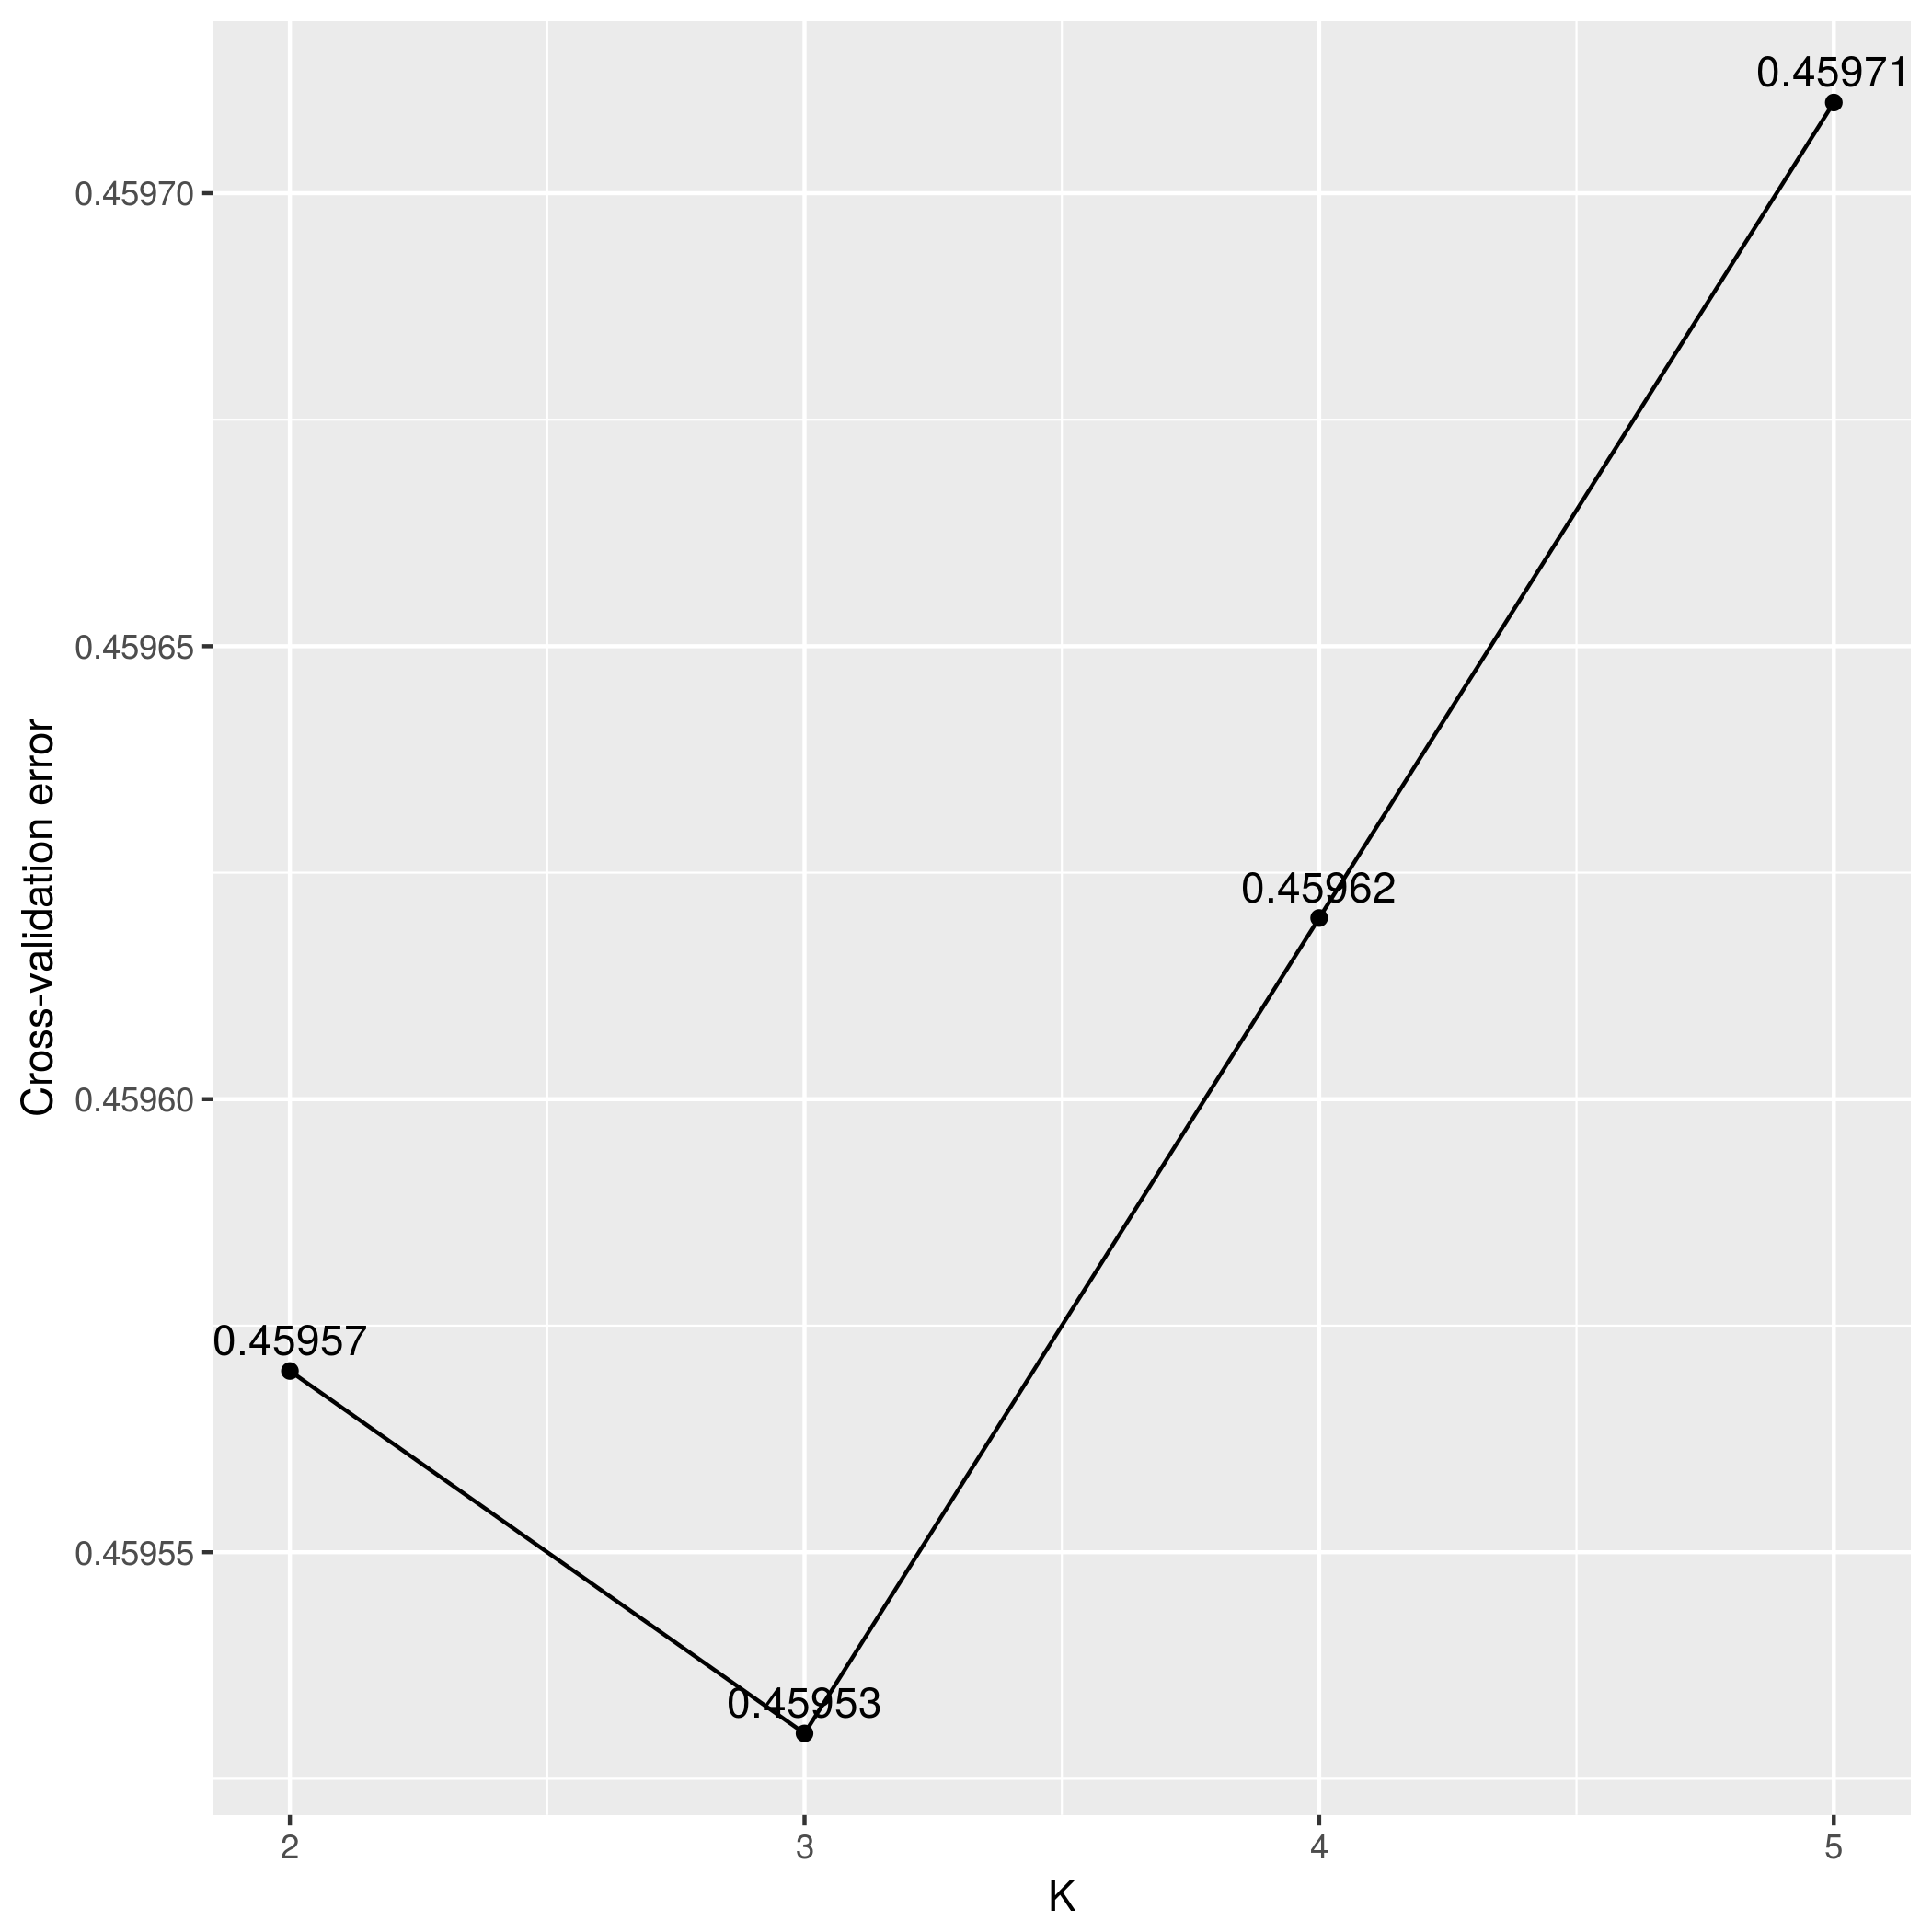
\includegraphics[scale = 0.5]{K5.png}
  \caption[Estimaci\'on de n\'umero de poblaciones]{Estimaci\'on de K, n\'umero de poblaciones posibles en la base de datos CHIBCHA.}
  \label{fig:k}
\end{figure}


\begin{table}[H]
  \centering
  \begin{tabular}{|l|l l|}
    \hline \hline
    & pob0& \\
    \hline
    pob0&&\\
    pob1&0.109&\\
    \hline \hline
  \end{tabular}
  \caption{Fst divergencia entre las poblaciones estimadas para K=2}
\end{table}

\begin{table}[H]
  \centering
  \begin{tabular}{|l| l l|}
    \hline \hline
    & pob0& pob1\\
    \hline
    pob1&0.017&\\
    pob2&0.121&0.082\\
    \hline \hline
  \end{tabular}
  \caption{Fst divergencia entre las poblaciones estimadas para K=3}
  \label{table:k3}
\end{table}

\begin{table}[H]
  \centering
  \begin{tabular}{|l| l l l|}
    \hline \hline
    & pob0& pob1&pob2\\
    \hline
    pob1&0.035& &\\
    pob2&0.089&0.061&\\
    pob3&0.119&0.078&0.015\\
    \hline \hline
  \end{tabular}
  \caption{Fst divergencia entre las poblaciones estimadas para K=4}
\end{table}



\begin{table}[H]
  \centering
  \begin{tabular}{|l| l l l l|}
    \hline \hline
    & pob0& pob1&pob2&pob3\\
    \hline
    pob1&0.067& & &\\
    pob2&0.050&0.055& &\\
    pob3&0.017&0.082&0.058&\\
    pob4&0.92&0.041&0.057&0.121\\
    \hline \hline
  \end{tabular}
  \caption{Fst divergencia entre las poblaciones estimadas para K=5}
\end{table}

Las tablas de divergencias nos muestran la separaci\'on entre las poblaciones estimadas. En este caso en particular se enfoca en la tabla \ref{table:k3} donde se observa que la poblaci\'on 2 y la poblaci\'on 0 tienen el valor de correlaci\'on m\'as alta, lo cual puede indicar que en estas poblaciones existen alelos iguales proviniente de una poblaci\'on ancestral.\\

Por otro lado, en la figura \ref{fig:an} podemos observar la derivaci\'on de las tres poblaciones utilizadas para este estudio (española, m\'exicana y africana). De manera similar podemos visualizar que la mayor\'ia de los individuos tienen poca frecuencia de la poblaci\'on africana, esto comprueba lo que se viene observando a trav\'es de la historia de la conquista en M\'exico.\\

\begin{figure}[H]
  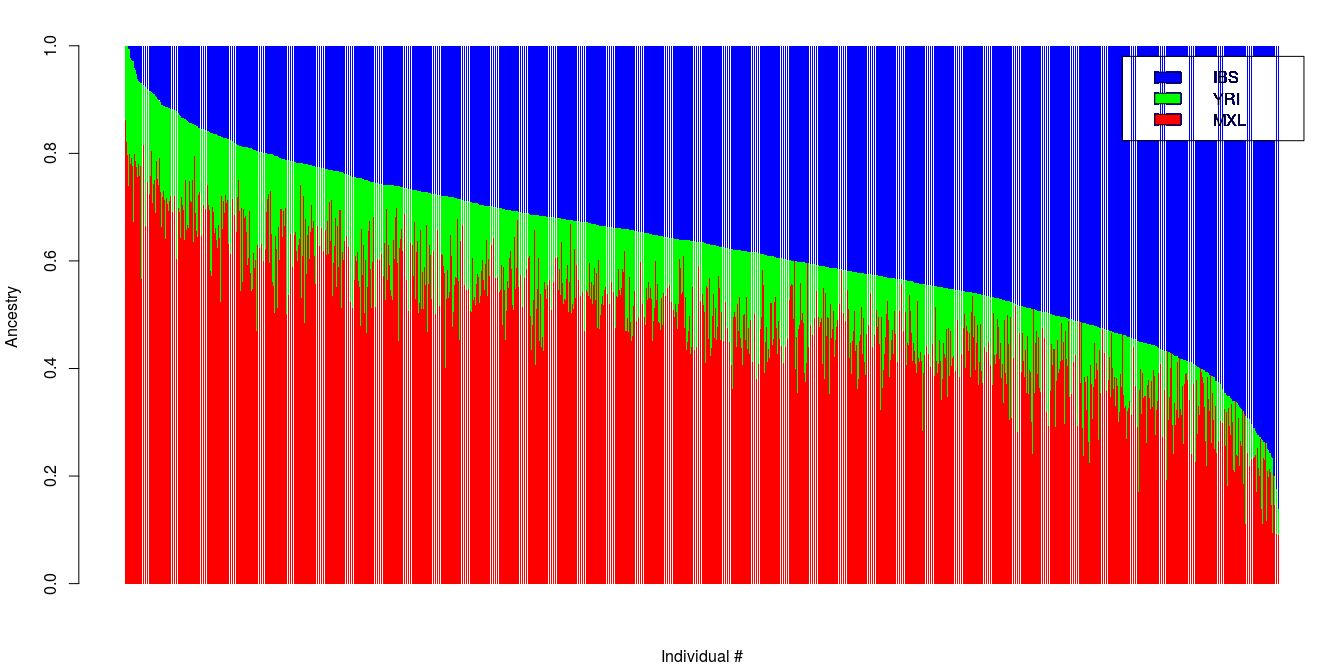
\includegraphics[scale=0.3]{Pro.png}
  \caption[Mapa de color para casos y controles]}{An\'alisis individual de ancestr\'ia total (casos y controles). Cada individuo es representado por una barra vertical en la gr\'afica.}
  \label{fig:an}
\end{figure}

\begin{figure}[H]
  \centering
  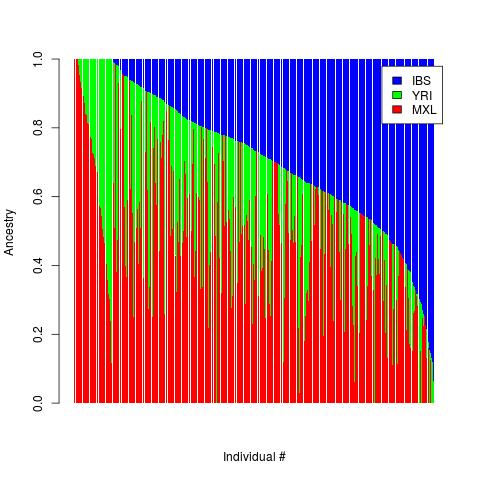
\includegraphics[scale=0.7]{rplot.jpg}
  \caption[Mapa de color para casos]{An\'alisis individual de ancestr\'ia para casos. Cada individuo es representado por una barra vertical en la gr\'afica.}
  \label{fig:ca}
\end{figure}

La figura \ref{fig:ca} tiene individuos con $100\%$ ancestralidad mexicana y casos de individuos sin ningún porcentaje de genes con ancestralidad mexicana. Adem\'as de mostrar una diferencia, con respecto al crecimiento del color verde (poblaci\'on africana), con la figura \ref{fig:an}. Esto puede deberse a que los casos provienen de entidades como Veracruz o Guerrero dado porcentaje de ancestrilidad altos de la poblaci\'on ancestral africana. De manera similar, dado que los individuos no muestran un distribuci\'on heterog\'enea de colores, puede inferirse que la relaci\'on con genes asociados al c\'ancer colorrectal estar\'a distribuido equitativamente en las tres poblaciones. 


\begin{figure}[H]
  \centering
  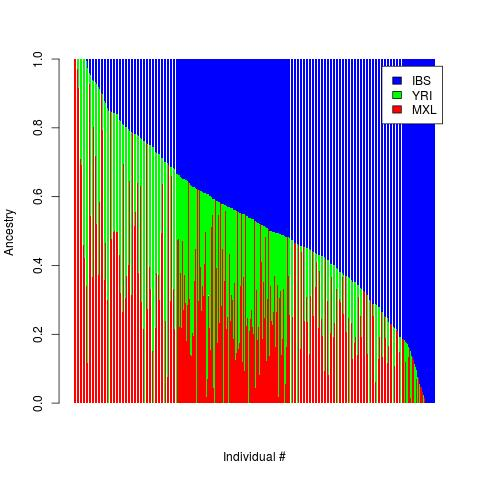
\includegraphics[scale=0.7]{r_malesplot.jpg}
  \caption[Mapa de color para casos masculino]{An\'alisis individual de ancestr\'ia para casos en g\'enero masculino. Cada individuo es representado por una barra vertical en la gr\'afica.}
  \label{fig:cam}
\end{figure}


\begin{figure}[H]
  \centering
  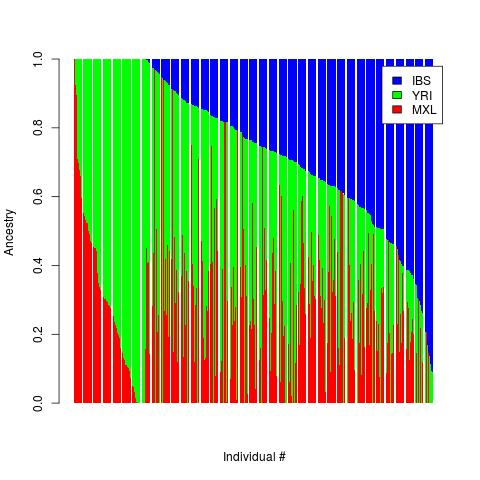
\includegraphics[scale=0.7]{r_femalesplot.jpg}
  \caption[Mapa de color para casos femenino]{An\'alisis individual de ancestr\'ia para casos en g\'enero femenino. Cada individuo es representado por una barra vertical en la gr\'afica.}
  \label{fig:caf}
\end{figure}


Con respecto a la posici\'on g\'enetica de los genes, y observando a cada indivudo en la gr\'afica \ref{fig:ca}, se obtuvo lo siguiente,\\

\begin{table}[H]
  \centering
  \begin{tabular}{|c|c|c|}
    \hline
    SNP & Locaci\'on& Poblaci\'on g\'enetica (\%)\\
    \hline
    rs74382455 & 1:84373659& Africana = 0.90\\
    rs2598121 & 7:37936286 & MXL = 0.96\\
    rs7311395 & 12:43574178 & Europea = 0.86\\
    rs7197593 & 16:55405713 & Europea = 0.97\\
    \hline
  \end{tabular}
\end{table}

De cuatro SNPs evaluados, dos de ellos tienen mayor porcentaje de poblaci\'on g\'enetica en españoles. Esto no implica que la poblaci\'on ancestral europea sea la de mayor correlaci\'on, si no que en estos cuatros SNPs tuvieron mayor relaci\'on. Puede ser que en los otros SNPs que no se mapearon pueda existir una ventaja de la misma poblaci\'on europea u otra de las dos.\\

Con respecto a las figuras \ref{fig:cam} y \ref{fig:caf} se puede observar que en el cuadro del g\'enero femenino existen mujeres con un porcentaje del 100 en genes con ascedencia \'africana, de manera similar, se puede observar que en el cuadro de hombres, hay individuos con porcentajes de 100 en ascedencia europea, esto siendo muy marcado en los distintos cuadros. 
   % ~20 páginas - Presentar los resultados tal cual son, y analizarlos.
\chapter{Conclusiones y futuros trabajos}

En la actualidad, el c\'omputo y las herramientas estad\'isticas forman gran parte para entender el comportamiento del mundo y de la vida. Los resultados que hemos encontrado, en colaboraci\'on con el Laboratorio Nacional de Medicina en Sistemas y el equipo de trabajo de Uruguay, han descrito un antecedente en la b\'usqueda de respuestas antes enfermedades como el c\'ancer que son un gran problema en el sector de salud nacional.\\

Los SNPs mencionados est\'an divididos en las tres poblaciones, pero muestran mayor actividad en la poblaci\'on europea, b\'asicamente en la española. Esto puede implicar que los genes asociados al c\'ancer colorrectal tiene un relaci\'on con la ascedencia europea,  dado el mestizaje en M\'exico, aunque como se mencion\'o en el apartado de resultados, falta observar el comportamiento de los otros SNPs que no se mapearon y dar un resultado m\'as completo. Por otro lado, siendo que en los cuadros \ref{fig:caf} y \ref{fig:cam} se ve una diferencia en porcentaje de genes para cada poblaci\'on, es notable mencionar que hay mujeres con ascedencia americana nativa al 100\% y de manera similar con ascedencia africana pero no existe ning\'un individuo con ascedencia europea; esto puede implicar que tal vez exista una relaci\'on mayor de la enfermedad con estas poblaciones, pero este no es el caso.\\

Estos an\'alisis tienen como objetivo dar una explicaci\'on m\'as contudente, aunque es necesario recalcar la complejidad computacional que esta presenta, ya que las bases de datos son de alta dimensionalidad y su an\'alisis generan problemas complejos. Por otro lado, es interesante notar que de los doce SNPs con mayor asociaci\'on al c\'ancer solo se pudieron observar cuatro, esto puede resolverse en la forma de generar mayores estudios en la parte g\'enetica poblacional aqu\'i en M\'exico y tener antecedentes que nos ayuden a entender el por que de las enfermedades. \\

\section{Futuros trabajos}

Aunque se ha generado un gran avance en la estimaci\'on de la ancestr\'ia en un conjunto de datos de genes con poblaciones desconocida, es necesario recalcar que este tipo de an\'alisis no indica con precisi\'on la cercania de la relaci\'on de la ancestria con el c\'ancer ya que se tiene un rango en la posici\'on g\'enetica provocando no conocer puntualmente la posici\'on del gen. Por lo tanto, en un trabajo futuro se recomienda comenzar a trabajar con an\'alisis de haploides el cu\'al puede generar mayor referencia en los asuntos de precisi\'on para relacionar las enfermedades con los genes.







            % ~5 páginas - Resumir lo que se hizo y lo que no y comentar trabajos futuros sobre el tema
\listoffigures              % Genera el ínidce de figuras, comentar línea si no se usa
\listoftables               % Genera índice de xtablas, comentar línea si no se us

%%%%%%%%%%%%%%%%%%%%%%%%%%%%%%%%%%%%%%%%%%%%%%%%%%%%%
%                   APÉNDICES                      %
%%%%%%%%%%%%%%%%%%%%%%%%%%%%%%%%%%%%%%%%%%%%%%%%%%%%%

%\appendix
%
%% this file is called up by thesis.tex
% content in this file will be fed into the main document
\chapter{Código/Manuales/Publicaciones}
% top level followed by section, subsection

\section{Apéndice}

Apéndice
               %Colocar los circuitos, manuales, código fuente, pruebas de teoremas, etc.

%%%%%%%%%%%%%%%%%%%%%%%%%%%%%%%%%%%%%%%%%%%%%%%%%%%%%
%                   REFERENCIAS                    %
%%%%%%%%%%%%%%%%%%%%%%%%%%%%%%%%%%%%%%%%%%%%%%%%%%%%%
% existen varios estilos de bilbiografía, pueden cambiarlos a placer
%\bibliographystyle{IEEEannot}
\bibliographystyle{acm} % otros estilos pueden ser abbrv, acm, alpha, apalike, ieeetr, plain, siam, unsrt

%El formato trae otros estilos, o pueden agregar uno que les guste:
%\bibliographystyle{Latex/Classes/PhDbiblio-case} % title forced lower case
%\bibliographystyle{Latex/Classes/PhDbiblio-bold} % title as in bibtex but bold
%\bibliographystyle{Latex/Classes/PhDbiblio-url} % bold + www link if provided
%\bibliographystyle{Latex/Classes/jmb} % calls style file jmb.bst

\bibliography{Bibliografia/biblio}             % Archivo .bib

\end{document}
